%!TEX root = ../thesis.tex

\subsection{Companion injection-recovery}
\label{subsec:injection-recovery}
To determine the detection limits for this method we employ an injection-recovery approach.
We take the observed spectra and inject onto them a synthetic companion, at the absolute flux ratio to which it would have been added to a synthetic host with the same parameters.
The injected companion {RV} is set to 100\kmps{} so that the companion lines are well separated from the lines of the host.
This separation chosen is slightly larger than what we have with our observations, \({rv}_{2}\) given in \cref{tab:observations}.

We restrict the search space by fixing the host parameters \(\teffsub{1}\) and \(\logg{}_{1}\) to those recovered fitting the non-injected spectra by a single component model.
The wavelength masking is used to reduce the level of mismatch between synthetic and observed spectra.

We apply the recovery method developed above on the injected spectrum, leaving only the companion \(\teffsub{2}\) and \({rv}_{2}\) parameters free, to recover the injected companion.
We repeated this for injected companions with temperatures below 5000\K{}.

We also perform the injection-recovery with synthetic host spectra, representing each target.
The wavelength range of the synthetic spectra used for this is three sections interpolated to 1024 values in the wavelength span of detectors \#1, 2, and 3.
For each section, Gaussian noise is added at the level measured in the corresponding detector in the observation of the target being represented.

In \cref{fig:injectrecoveryhd30501} we show the results of the injection-recovery on {HD 30501}.
The blue dots represent the recovered companion temperature when injected into real observations, while the orange triangles represent injection into a synthetic host.
Error bars of \(\pm100\)\K{} are included to indicate the grid size, and do not come from the recovery itself.
The black dashed diagonal is the temperature 1:1 relation, where a correctly recovered companion should lie.

The grey shaded region indicates the \(\pm 1000\)\K{} temperature range explored for the injection-recovery of the companion.
This shows how the bounds of the grid are recovered at low temperatures.

For {HD 30501} the injection onto synthetic and observed spectra produce similar results.
At temperatures above 3800\K{}, in both the real and synthetic spectra, the injected companion is recovered within 100\K{}.
For injected companion temperatures below 3800\K{} the temperature recovered is systematically higher than the injected value.
This indicates that the companion is not correctly recovered and is affected by the added noise.
We determine this temperature to be the upper temperature limit for the recovery.
For the other stars we could not conclude on the upper limit due to spectral mismatch issues.
In these cases we use the results from the synthetic injection to derive a temperature recovery cut-off for each target, each simulated with the closest host star spectrum.

In \cref{fig:injection_shape} we show the minimum \textchisquared{} for each companion temperature in the recovery grid.
We do this for 7 different injected companion temperatures between 2500 and 4500\K{}.
For the higher temperature companions, the \textchisquared{} is parabolic in shape, recovering the correct temperature, as expected.
At lower temperatures there is a strong asymmetry in the \textchisquared{} with it flattening out on the lower temperature side.
The 1-, 2-, 3-\(\sigma\) values (with 2 degrees of freedom) of 2, 6 and 11 above the minimum \textchisquared{} are not shown in the bottom panel of \cref{fig:injection_shape} which is a close-up around the minimum \textchisquared{} as are indistinguishable in the top panel due to the \textchisquared{} y-scale.
The black vertical line indicates the 2300\K{} temperature limit of the {PHOENIX-ACES} models.

\begin{figure}
    \centering
    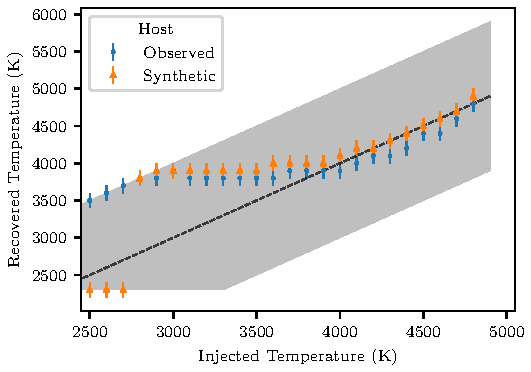
\includegraphics[width=0.6\linewidth]{figures/companion_recovery/inject_recovery_hd30501.pdf}
    \caption[Result of simulated injection-recovery of synthetic companions on {HD 30501}.]{Result of simulated injection-recovery of synthetic companions on {HD 30501}.
        The blue dots and orange triangles indicate the recovered companion temperature for the observed and synthetic spectra respectively.
        The \(\pm100\)\K{} error bars are the grid step of the synthetic models.
        The black dashed diagonal shows the 1:1 temperature relation.
        The grey shaded region indicates the \(\pm1000\)\K{} temperature range explored.
        Gaussian noise added to the synthetic spectra was derived from the observed spectra.}
    \label{fig:injectrecoveryhd30501}
\end{figure}


\begin{figure}
    \centering
    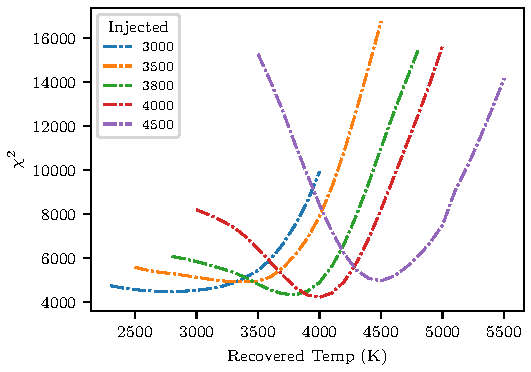
\includegraphics[width=0.7\linewidth]{figures/companion_recovery/chi2_shape_investigation}
    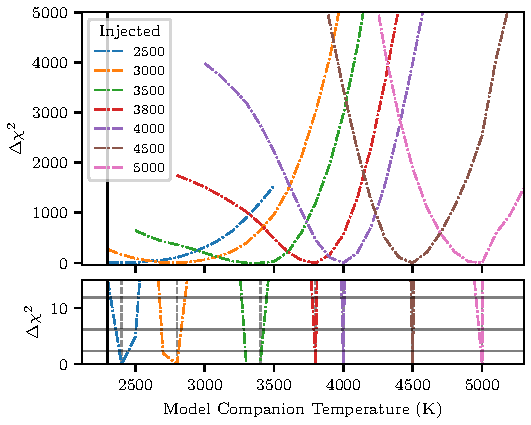
\includegraphics[width=0.7\linewidth]{figures/companion_recovery/chi2_shape_investigation_with_delta}
    \caption[Shape of simulated \textchisquared{} with different injected companion temperatures.]{Top: Companion temperature verses \textchisquared{} for simulations with different injected companion temperatures.
        Other fixed parameters for these fully synthetic simulations was \(\teffsub{1}=5200\)\K{}, \(\logg_{1}=4.5\), \(\logg{}_{2}=5.0\), and both \feh{}=0.0.
        A fixed Gaussian noise corresponding to a \snr{} of 300 was used.
        Bottom: A close up view of \textchisquared{} < 15.
        The three horizontal grey lines indicate the 1-, 2-, 3-$\sigma$ with 2 degrees of freedom.
        The vertical dotted lines indicate the location of the minimum \textchisquared{} recovered for each companion.
        The black solid vertical in both panels shows the 2300\K{} cut-off of the {PHOENIX-ACES} models}
    \label{fig:injection_shape}
    %\label{fig:chi2shapeinvestigation}
\end{figure}

%!TEX root = ../thesis.tex
\begin{table}
       \centering
  \begin{threeparttable}

       \caption{Upper mass limits of target companions assuming a companion \logg{}=5.0. Masses are derived from~\citet{baraffe_new_2015} evolutionary models using \(\teff{}\) and \logg{}. The flux ratio \(\rm F_2/F_1\) is  the absolute flux ratio between the cut-off temperature and the target host star.}

        \begin{tabular}{l c c c}
            \toprule
            Target & \txteff{} cut-off (K) & \(\rm F_2/F_1\) & Mass limit (\Mjup{})\\
            \midrule
            {HD 4747}     &  3\,900 & 0.084 & 598 \\
            {HD 162020} & 3\,900 & 0.147 & 598 \\
            {HD 167665} & 3\,800 & 0.054 & 560 \\
            {HD 168443} & 4\,000 & 0.094 & 618 \\
            {HD 202206} & 3\,900 & 0.075 & 598 \\
            {HD 211847} & 3\,900 & 0.079 & 598 \\
            {HD 30501}   & 3\,800\tnote{a} & 0.106 & 560 \\
            \bottomrule
        \end{tabular}
        \label{tab:mass_limits}
        \begin{tablenotes}[flushleft]
            \small
                \item [a] {From observed spectra }
        \end{tablenotes}
  \end{threeparttable}

\end{table}



Using the temperature cut-off values, we derive an upper mass limit for the companions around our stars using the~\citet{baraffe_new_2015} evolutionary models, finding the closest point matching the spectral temperature cut-off and \(\logg{}=5.0\).
These values are given in \cref{tab:mass_limits} and are between 560 and 618~\Mjup{}.
The flux ratio between the cut-off and the host star are also provided for, being between 5 and 15\% in this wavelength span.

